\chapter{Fundamentação teórica}

\section{Considerações iniciais}
Neste capítulo introduzimos os conceitos que serão abordados durante o desenvolvimento deste trabalho. A seção~\ref{sec:arquiteturas} traz uma explanação sobre as arquiteturas que os protocolos abordados neste trabalho fazem uso. A Seção~\ref{sec:protocolos} apresenta uma visão geral sobre cada um dos protocolos utilizados bem como seu funcionamento e características.

\section{Arquiteturas}
\label{sec:arquiteturas}

De modo geral existem dois principais padrões para transmissão de mensagens na camada de aplicação entre computadores conectados em rede, são eles: requisição-resposta (do inglês, request-response) e publicação-assinatura (do inglês, publish-subscribe).

\subsection{Requisição-Resposta}

O padrão requisição-resposta funciona da seguinte forma, um computador envia uma requisição de algum dado através de um canal, nesse caso a rede, e um outro computador recebe essa requisição, processa esse recebimento e envia uma resposta de volta \cite{livro_hohpe2003_enterpriseIntegrationPattern}. Esse procedimento é análogo a uma ligação telefônica, em que uma pessoa, requisitante, liga solicitando alguma informação através de um canal, nesse caso a rede de telefonia, e outra pessoa responde, atendendo essa solicitação.

Esse padrão é extremamente comum na Internet hoje, pois é o padrão utilizados pelos navegadores. Quando uma pessoa digita uma URL num navegador, este faz uma requisição utilizando o protocolo HTTP, que será detalhado mais adiante, a um servidor e este por sua vez, ao receber a requisição, processa e geralmente devolve como resposta um texto no formato HTML que é interpretado pelo navegador e utilizado para renderizar a página em questão \cite{url_mozilla2018_httpOverview}

Na extensa maioria dos casos este padrão é implementados de forma síncrona, ou seja, ao realizar uma requisição, o requisitante permanece esperando até obter uma resposta do destinatário ou até o período máximo de espera (timeout) ser atingido. Entretanto, em alguns casos, este padrão pode ser implementado de forma assíncrona, ou seja, não há necessidade de espera por parte do solicitante após a realização da requisição. Neste caso cabe ao destinatário da solicitação entrar em contato com o requerente para devolver-lhe o resultado do seu requerimento FONTE: \url{ https://www.w3.org/Protocols/HTTP/1.1/rfc2616bis/draft-lafon-rfc2616bis-03.html#rfc.section.1}. Um exemplo de requisição assíncrona é o envio de email, onde não é necessário que o remetente permaneça esperando uma resposta do destinatário.

\subsection{Publicação-Assinatura}

No padrão publicação-assinatura, ao contrário do padrão requisição-resposta, a troca de mensagens entre o remetente e o destinatário não ocorre de forma direta. Neste padrão existem 3 agentes, o publicador, o assinante e a central. 

A comunicação entre os agentes ocorre da seguinte forma: o publicador envia sua mensagem para a central contendo o conteúdo da mensagem e o tópico ou categoria da mensagem. O assinante, por sua vez, envia para a central uma solicitação de assinatura para um determinado tópico ou categoria. É permitido ao assinante possuir quantas assinaturas quiser. A central funciona como um intermediário e é responsável por receber mensagens de publicadores e por aceitar e registrar solicitações de assinaturas. Ao receber uma mensagem de um publicador, a central verifica quantos e quais são os assinantes do tópico daquela mensagem e então os envia a referida mensagem. 

As duas principais vantagens desse padrão são a independência e a escalabilidade. Independência pois não existe nenhuma correlação entre publicadores e assinantes, eles não precisam ter conhecimento da existência um do outro, inclusive é factível a presença de publicadores de um determinado tópico sem que hajam assinantes e vice-versa. A escalabilidade refere-se a potencial de crescimento da rede através da inclusão nós, seja elem publicador ou assinante, neste tipo de rede. Não se faz necessário alterações na topologia da rede para adição ou remoção de um nó, pois o padrão já dá suporte a este tipo de operação.

\section{Protocolos}
\label{sec:protocolos}
Neste trabalho vamos utilizar um total de 6 protocolos mais difundidos para comunicação M2M (Machine-to-Machine). São eles:
\begin{enumerate}
\item HTTP
\item CoAP
\item MQTT
\item AMQP
\item STOMP
\item XMPP
\end{enumerate}

\subsection{HTTP}

\subsubsection*{O que é ?}
O Hypertext Transfer Protocol (HTTP), ou Protocolo de Transferência Hipertexto em português, é um protocolo de comunicação, localizado na camada de aplicação (a última camada no modelo OSI). Ele é utilizado em sistemas de informação com o objetivo de transmitir documentos em hipermídia, distribuídos e colaborativos. Hipermídia é a reunião de vários tipos de mídias, tais como imagens, vídeos, sons e texto, em um documento no ambiente computacional, que são navegáveis, interativos e cuja leitura se dá de forma não linear. Qualquer página na Web é um ótimo exemplo de um documento de hipermídia. 

O desenvolvimento do HTTP é coordenado pela World Wide Web Consortium (W3C) e pela Internet Engineering Task Force (IETF) e tem sido a principal forma de comunicação na World Wide Web desde que foi criado, em 1990. Na sua primeira versão HTTP/0.9, seu único objetivo era a transferência simples de dados através da internet. Na sua segunda versão, a 1.0, o procotolo foi melhorado, foi incluído os headers, que continham informações sobre o que estava sendo trafegado. Também foi incluído nesta versão o modelo request-response, ou requisição-resposta, para informar se a comunicação foi realizada com sucesso ou não. Atualmente o HTTP está na versão 2.0 e diversas melhorias foram acrescidas, como compressão de headers, definição de prioridade nas requisições, entre outas.

\subsubsection*{Características}
Com relação as características do HTTP, pode-se dizer que ele é:
\begin{itemize}
\item Simples: as mensagens em HTTP foram desenhadas para serem fáceis de ler e entender por humanos sem necessitar de nenhum tipo de aparato extra;
\item Extensível: os cabeçalhos das mensagens HTTP foram criados de forma a propiciar a adição de novas propriedades de maneira fácil e intuitíva;
\item Stateless: o protocolo foi criado para não manter estado, ou seja, cada requisição é totalmente independente uma da outra. Não há compartilhamento de dados entre duas requisições diferentes.
\item Confiabilidade: Como HTTP envia seus dados através da camada de transporte TCP/IP, ele é um protocolo considerado seguro, pois os dados trafegados não se perdem "silenciosamente". 
\end{itemize}


\subsubsection*{Como funciona ?}
O HTTP funciona no modelo request-response utilizando uma arquitetura cliente-servidor. Quando nós abrimos um Web Browser, como Google Chrome, Mozilla Firefox ou Internet Explorer e digitamos uma URL, esse navegador é o cliente da nossa arquitetura e ele está fazendo uma requisição HTTP a uma aplicação hospedada em um computador em outra parte do globo, que é o servidor. Esse servidor, por sua vez, ao receber essa requisição, realiza o processamento desta e retorna uma resposta ao cliente. Essa resposta contém informações sobre este processamento e pode ou não conter o conteúdo solicitado no corpo da mensagem.

As mensagens trocadas entre o cliente e o servidor http possuem uma estrutura predefinida. Essa estrutura é constituída por 3 partes, a Request-Line, ou linha inicial, o Header, ou cabeçalho, e o Body, ou corpo da mensagem. 
A Request-line é a primeira linha da requisição. Caso esta seja uma solicitação enviada pelo cliente, nós temos o tipo de método da solicitação e a versão do protocolo que estamos utilizando. Caso seja uma resposta do servidor, nós temos a versão do protocolo seguido pelo código da resposta da mensagem. Os códigos mais comuns são: 200 - indica que a solicitação foi processada com sucesso, 400 - indica que a requisição está com algum erro de sintaxe, 401 - indica que está tentando acessar um recurso cuja permissão é restrita e é necessário informar alguma credencial, 403 - indica que a requisição é válida, e que o usuário foi autenticado, mas não possui permissão para acessar o recurso, 404 - indica que o recurso que está sendo solicitado não foi encontrado. 
Da segunda linha em diante vem o Header, que contém uma série de informações sobre a requisição em si, tais como data/hora, endereço e tipo do servidor, tamanho e tipo do conteúdo de retorno da resposta, entre outros.
Após o término do Header, vem uma linha em branco e em seguida vem o body, que é opcional, com o conteúdo da mensagem em si. Quando acessamos uma URL, é no body que o servidor manda o arquivo html que é renderizado na tela do browser.

O HTTP utiliza uma série de métodos para indicar qual é a ação desejada pelo cliente ao servidor. São ao todo 9 métodos, mas 4 são os mais utilizados, são eles: GET, POST, PUT e DELETE. Cada um deles possui uma semântica própria, mas eles compartilham algumas características em comum. Abaixo segue uma breve descrição do que cada método faz.
\begin{itemize}
\item GET: é um método responsável por buscar informações. Esse método pode ou não ter conteúdo no corpo da resposta;
\item HEAD: é um método idêntico ao GET, porém não poussui conteúdo no corpo da resposta;
\item POST: é um método responsável por submeter informações ao servidor. Normalmente é utilizado para causar mudanças de estados no mesmo;
\item PUT: também é um método de submissão, porém é comumente utilizado para atualizar informações já presentes no servidor;
\item DELETE: é responsável por deletar recursos específicos;
\item CONNECT: é responsável por criar um túnel de conversasão entre o cliente e o servidor. Normalmente requer algum tipo de autenticação por parte do cliente;
\item OPTIONS: é usado para obter as opções de requisição permitidas para um determinado recurso no servidor;
\item TRACE: é utilizado para obter o caminho que a requisição faz até o servidor. É retornado para o cliente quais proxys e máquinas a sua requisição passa até chegar ao destino;
\item PATCH: é um método utilizado para realizar alterações parciais em um derterminado recurso;
\end{itemize}


FONTES:
\url{https://pt.wikipedia.org/wiki/Hypertext_Transfer_Protocol}
\url{https://developer.mozilla.org/en-US/docs/Web/HTTP/Overview}
\url{https://developer.mozilla.org/en-US/docs/Web/HTTP/Status}
\url{https://www.digitalocean.com/community/tutorials/how-to-troubleshoot-common-http-error-codes}
\url{https://hpbn.co/brief-history-of-http/}
\url{https://en.wikipedia.org/wiki/Hypertext_Transfer_Protocol}
\url{https://developer.mozilla.org/en-US/docs/Web/HTTP}
\url{https://developer.mozilla.org/en-US/docs/Web/HTTP/Methods}
\url{https://www.w3.org/Protocols/rfc2616/rfc2616.html}
\url{https://developer.mozilla.org/en-US/docs/Web/HTTP/Resources_and_specifications}
\url{https://www.w3.org/Protocols/Specs.html}
\url{https://www.w3.org/Protocols/HTTP/1.1/rfc2616bis/draft-lafon-rfc2616bis-03.html#rfc.section.1}
\url{https://pt.wikipedia.org/wiki/Hiperm%C3%ADdia}
\url{https://pt.wikipedia.org/wiki/Design_de_hiperm%C3%ADdia}


\subsection{CoAP}

\subsubsection*{O que é ?}
O Constrained Application Protocol (CoAP) é um protocolo para web da camada de aplicação, criado pela Internet Engineering Task Force (IETF)  especificamente para ser utilizado na comunicação entre máquinas (Machine-to-machine ou M2M) que sejam por elas mesmas limitadas, como disporem de uma fonte de energia restrita ou possuírem baixo poder de processamento ou armazenamento, ou estejam imersos em redes limitadas ou que possuam restrições de alguma forma, seja por uma alta taxa de perda de pacotes, ou por uma baixa velocidade de banda ou por qualquer outro motivo.	

\subsubsection*{Características}
Por ter sido criado no modelo REST, uma das grandes vantagens de se utilizar o CoAP é a integração facilitada com o protocolo HTTP, que é o protocolo mais utilizado na web. Outra característica importante deste protocolo é possuir um cabeçalho pequeno, limitado a 4 bytes, resultando numa diminuição do tamanho do pacote como um todo e na priorização do conteúdo da mensagem em si. Este cabeçalho é constituído de, entre outras coisas, um identificador da mensagem, um token e um tipo da mensagem. O identificador serve para o CoAP detectar mensagens em duplicidade. O Token por sua vez, permite o CoAP relacionar as mensagens de requisição com a sua resposta. O tipo de mensagem pode variar entre confirmable ou confirmável (CON), Non-confirmable ou não-confirmável (NON), acknowledgement ou recebido (ACK) e reset ou resetar (RST). Esta tupla de id, token e tipo tornam possível uma outra característica fundamental do CoAP que é o suporte a mensagens assíncronas, ou seja, o cliente pode fazer uma requisição ao servidor, e este por sua vez não responder imediatamente e sim depois de um certo tempo. Algumas outras características do CoAP incluem o suporte a descoberta, suporte multicast e suporte a content-type, do mesmo modo que o HTTP. 

\subsubsection*{Como funciona ?}
Como o CoAP foi criado baseado no modelo REST, funciona de maneira muito similar ao HTTP. Na troca de mensagens existe um servidor que disponibiliza recursos através de uma URL, e um cliente, que acessa esses recursos fazendo uma requisição a esta URL utilizando os mesmos métodos do HTTP: GET, POST, PUT e DELETE. Porém ao contrário do HTTP, o CoAP foi desenvolvido utilizando UDP na camada de transporte, e por isso necessitou implementar seus próprios métodos de detecção de duplicidade, retransmissão de pacotes e confiabilidade. Para tratar a confiabilidade o CoAP se utiliza do tipo de mensagem CON. Quando um nó (cliente ou servidor) envia uma requisição deste tipo, ele espera receber um outra requisição do tipo ACK como resposta, informando que o outro lado recebeu a requisição enviada. A figura \ref{fig:coap_success} ilustra uma requisição CoAP do tipo CON feita por um cliente utilizando o método GET solicitando o valor da temperatura. Na requisição da esquerda a temperatura é retornada com sucesso pelo servidor no conteúdo mensagem ACK. Na requisição da direita, é retornado o erro 404 informando que o recurso solicitado não foi encontrado.

\begin{figure}[h]
\centering
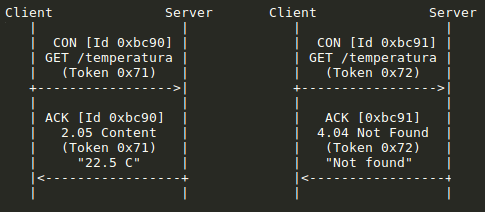
\includegraphics[height=5cm]{figuras/coap_request_success.png}
\caption{Exemplo de requisição CoAP do tipo CON e da resposta ACK}
\label{fig:coap_success}
\end{figure}

Caso o outro lado não devolva esta mensagem esperada, o nó solicitante  aguarda o tempo de timeout definido e então envia novamente a mensagem CON, e continua reenviando até receber a resposta ACK esperada. A figura \ref{fig:coap_timeout} ilustra o reenvio da requisição por parte do cliente após timeout até o recebimento da resposta ACK do servidor. Por outro lado, mensagens do tipo NON são não confirmáveis, ou seja, não necessita receber uma mensagem ACK como resposta.

\begin{figure}[h]
\centering
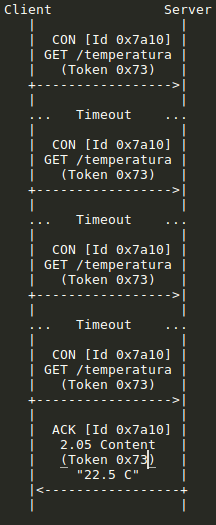
\includegraphics[height=13cm]{figuras/coap_request_timeout.png}
\caption{Exemplo de reenvio da requisição CoAP do tipo CON após o timeout}
\label{fig:coap_timeout}
\end{figure}

Como já mencionado anteriormente, o CoAP faz uso de um token no cabeçalho para possibilitar o envio de mensagens assíncronas. Este token é utilizado para relacionar as mensagens. Quando um cliente envia uma requisição para um servidor requisitando um recurso, seja ela do tipo CON ou NON, nesta requisição há um token, e o servidor, ao responder, faz uso deste mesmo token na mensagem de resposta. Caso a mensagem solicitada seja CON e o servidor não puder enviar o conteúdo da resposta imediatamente, ele envia uma mensagem ACK vazia e, após algum tempo, envia a resposta também utilizando o mesmo token inicial. A figura \ref{fig:coap_token} ilustra bem a situação mencionada acima.

\begin{figure}[h]
\centering
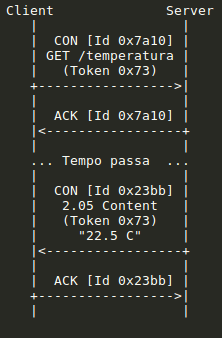
\includegraphics[height=8cm]{figuras/coap_request_token.png}
\caption{Exemplo de uso do token relacionando diferentes requisições CoAP}
\label{fig:coap_token}
\end{figure}

FONTES
http://coap.technology/
https://tools.ietf.org/html/rfc7252


\subsection{MQTT}

O Message Queuing Telemetry Transport (MQTT) é um protocolo de comunicação entre máquinas (M2M ou Machine-to-Machine) e foi desenhado em cima de certos princípios que o torna ideal para ser utilizado em aplicações para Internet das Coisas. Os princípios que o MQTT se baseia são de minimizar a quantidade de banda consumida e de recursos utilizados do dispositivo em que está rodando, tentando manter a confiabilidade e assegurar que a mensagens serão entregues com sucesso. Ele é um protocolo extremamente leve que funciona usando uma arquitetura publish-subscribe para enviar e receber mensagens. Ele é bastante eficiente quando utilizado em ambientes onde a rede é de baixa qualidade e/ou quando é necessário que as mensagens transmitidas contenham a menor quantidade possível de dados "extras", para que cada pacote de dados enviados possa ser aproveitado ao máximo.

\subsubsection*{Características}

Dentre as características do MQTT estão o fato dele utilizar os protocolos TCP/IP para transmitir suas mensagens, garantindo desse modo a não perda de pacotes durante a transmissão dos dados. Além disso ele utiliza a arquitetura publicação-assinatura, que provê para ele uma distribuição de mensagens de um para muitos, ou seja, um publica e vários recebem. Ademais o protocolo minimiza a sobrecarga durante a troca de mensagens no intento de reduzir a quantidade de dados enviados na rede. 

Outra característica importante do MQTT refere-se a qualidade do serviço durante a entrega das mensagens aos assinantes. Ele dispões de 3 tipos de serviços de entrega de mensagens: "no máximo 1", "pelo menos 1" e "exatamente 1". "No máximo 1" que dizer que a mensagem tentará ser entregue 1 vez apenas e não haverá tentativa de reenvio caso haja perda. "Pelo menos 1" quer dizer que a mensagem será entregue, porém pode haver duplicidade, ou seja, a mesma mensagem enviada mais de uma vez. "Exatamente 1" quer dizer que há garantia que a mensagem será entregue e que não haverá duplicidade.

FONTE: http://docs.oasis-open.org/mqtt/mqtt/v3.1.1/os/mqtt-v3.1.1-os.html

\subsubsection*{Como funciona}


FONTE:
\url{http://mqtt.org}


\subsection{AQMP}

\subsubsection*{O que é?}
AMQP ou Advanced Message Queuing Protocol é um padrão aberto para envio de mensagens utilizando filas criado em 2003. Ele foi criado para prover a troca de mensagens de forma eficiente entre uma gama de aplicações e padrões de comunicação diferentes. 


\subsection{STOMP}

\subsubsection*{O que é?}

STOMP deriva do acrônimo em inglês Simple Text Oriented Message Protocol, ou Protocolo Orientado a Mensagens de Texto Simples em tradução livre. Sua criação foi baseado no protocolo HTTP no que tange ao escopo das mensagens, porém a troca de mensagens utiliza o padrão publicação-assinatura. Por ter sido criado nos moldes HTTP, este protocolo também possui os mesmo agentes: um Cliente e um Servidor. Este protocolo foi criado através da necessidade de se conectar a centrais de mensagens empresariais utilizando linguagens orientadas a script como Python, Ruby e Perl, visando prover o câmbio de mensagens assíncronas da forma mais básica e simples possível \cite{url_stomp2018_stompSpecification}. 


\subsubsection*{Como funciona ?}

No STOMP a comunicação é baseada em frames, tendo como modelo as requisições do HTTP. Um frame é constituído de três partes: o comando, o cabeçalho e o corpo da mensagem. Tanto o cabeçalho quanto o corpo da mensagem são opcionais. A primeira linha do frame é o comando, que indica qual é a ação que será realizada, cujos valores possíveis são: CONNECT, SEND, SUBSCRIBE, UNSUBSCRIBE, BEGIN, COMMIT, ABORT, ACK, NACK e DISCONNECT. Da segunda linha em diante são os valores do cabeçalho, informados seguindo o modelo <chave>:<valor>, sendo um par chave:valor para cada linha. Após o fim do cabeçalho é colocada uma linha em branco para indicar o término do mesmo e a partir da linha seguinte começa o corpo da mensagem. Ao fim do corpo da mensagem é inserido uma linha com os caracteres \^{}@ para indicar o fim da mensagem. Abaixo estão dois exemplos de mensagens STOMP, a primeira com comando e cabeçalho, sem corpo, e a segunda com o corpo da mensagem.

\begin{lstlisting}{style=code, caption=Exemplo de mensagem com comando e cabeçalho}
CONNECT
accept-version:1.0,1.1,2.0
host:stomp.github.org

^@
\end{lstlisting}

\begin{lstlisting}{caption=Exemplo mensagem com comando, cabeçalho e corpo}
SEND
destination:/queue/a
content-type:text/plain

hello world to queue a.
^@
\end{lstlisting}

No STOMP, apesar do cabeçalho ser opcional, existem alguns casos, dependendo do tipo do comando da mensagem, em que se faz necessário informar alguns valores. No comando SEND por exemplo, é obrigatório informar o \textit{destination} com um valor contendo o destinatário da mensagem, como exemplificado no exemplo 2 da mensagem acima. Cabeçalhos obrigatórios, se não forem informados, obtém como resposta um mensagem do tipo ERROR. Abaixo um exemplo deste tipo de mensagem, que derivou de um envio de uma requisição mal formatada.

\begin{lstlisting}
ERROR
receipt-id:message-12345
content-type:text/plain
content-length:171
message: malformed frame received

The message:
-----
MESSAGE
destined:/queue/a
receipt:message-12345

hello world to queue a!
-----
Did not contain a destination header, which is REQUIRED
for message propagation.
^@
\end{lstlisting}

Há também alguns valores que não são obrigatórios entretanto são altamente recomendáveis estarem presentes no cabeçalho, como é o caso do  content-length e content-type nos tipo de mensagem SEND. Todavia a ausência destes valores no cabeçalho não é interpretado como um erro pelo servidor. 


\subsubsection*{Características}
No STOMP as principais características são flexibilidade e simplicidade. A estruturação e formatação das suas mensagens são bastante legíveis e o cabeçalho dos frames não contém dados desnecessários. Além disso o protocolo dá liberdade para acrescer informações no cabeçalho que não estão previstas na especificação. Outra característica importante é que o STOMP não restringe os tipos de comandos possíveis, ou seja, um cliente pode enviar uma mensagem com o comando FOWARD por exemplo, e, caso o servidor esteja preparado para receber este tipo de mensagem, ela será processada, caso contrário será retornado um ERROR.

Apesar de ser um protocolo simples, o STOMP dá suporte ao modelo transacional, ou seja, o processamento de diversos frames como uma única transação. Funciona da seguinte maneira: um cliente envia uma requisição do tipo BEGIN e, em seguida, envia uma série de requisições do tipo SEND. Ao final ele envia uma requisição do tipo COMMIT e então todas as requisições SEND enviadas anteriormente serão processadas como uma só. Para que este tipo de operação seja efetuada com sucesso é necessário informar no cabeçalho da mensagem BEGIN a chave \textit{transaction} com algum valor como id, e todas as mensagens SEND e COMMIT devem conter este cabeçalho com o mesmo id. Também é possível iniciar várias transações em paralelo, desde que mantenham id's diferentes. Qualquer transação que não tenham recebido COMMIT será abortada caso o cliente envie uma mensagem DISCONNECT ou ABORT ou caso a conexão TCP falhe por algum motivo.


\subsection{XMPP}
